\section{Weisfeler-Lehman}
\subsection{Definitions}
	\begin{definition}
		A \textit{partial ordering} of a set $S$ is a relation $<$ on $S$ satisfying the following for all $a,b,c$ in S:
		\begin{enumerate}
			\item Irreflexive: not $a<a$.
			\item Asymmetric: If $a<b$ then not $b<a$.
			\item Transitive: If $a<b$ and $b<c$ then $a<c$.
		\end{enumerate}
		For all $a,b\in S$, if $a<b$ or $b<a$, we say $a$ and $b$ are \textit{comparable}; otherwise,we say $a$ and $b$ are \textit{incomparable}.
	\end{definition}
	% Let $\mathfrak{X}$ be a set of graphs and $\mathcal{A}$ be an algorithm mapping $\mathfrak{X}$ to itself. 
	% \begin{definition}
	% 	An algorithm $\mathcal{A}$ is called \textit{canonical} if
	% 	\begin{enumerate}
	% 		\item for all $X\in\mathfrak{X}$ and for all $g\in$ Sym$(V(X))$ \[\mathcal{A}(gXg^{-1})=\mathcal{A}(X)\]
	% 	\end{enumerate}
	% \end{definition}
	% \begin{definition}
	% 	An algorithm is called \textit{canonical} if for all $G=(V,E)\in\mathfrak{X}$ where $X=A(G)$ and for all $g\in$ Sym$(V)$ \[\mathcal{A}(gXg^{-1})=\mathcal{A}(X)\]\cite{weisfeiler1976construction}.
        
	% \end{definition}
    % \begin{definition}
    %     A canonical algorithm $\mathcal{A}$ is called a \textit{canonization algorithm} if for any $G=(V,E)\in\mathfrak{X}$ where $X = A(G)$ there exists $g\in$ Sym$(V)$ such that \[\mathcal{A}(X)=gXg^{-1}\]\cite{weisfeiler1976construction}. 
    % \end{definition}
	% \begin{definition}
	% 	An algorithm $\mathcal{A}$ mapping $\mathfrak{X}$ into itself is called \textit{semi-invariant} if for any $G\in\mathfrak{X}$ where $X=A(G)$ and $G=(V,E)$, and for any $g\in$ Sym$(V)$ there exists $h\in$ Aut$(X)$ such that\[\mathcal{A}(gXg^{-1})=gh\mathcal{A}(X)h^{-1}g^{-1}\] where \[\text{Aut}(X)=\{h\in\text{Sym }(V):hXh^{-1}=X\}\]\cite{weisfeiler1976construction}. 
	% \end{definition}
	\begin{definition}
		Given a graph $G=\{V,E\}$, a \textit{canonical labeling} of $V$ is a partial ordering of $V$ such that if vertices $a$ and $b$ are incomparable, then there is a graph automorphism sending $a$ to $b$ \cite{weisfeiler1968}.
	\end{definition}
    \begin{definition}
        Given a graph $G=\{V,E\}$ and an algorithm $\mathcal{A}$ for obtaining a canonical labeling of $G$, a \textit{canonical form} of $G$ is its adjacency matrix, $A(G)$, with respect to a canonical labeling of its vertices, denoted $Canon_{\mathcal{A}}(G)$ \cite{weisfeiler1968}.
    \end{definition}
\subsection{A Canonization Algorithim}
WL is a classic and important method for partitioning the vertices of a graph $G$ based on the automorphism group of $G$ \cite{weisfeiler1968,weisfeiler1976construction}. Since the original 1968 paper, the power of WL has been improved. These improvements, called $k$-WL, where $k$ is called the dimension, can identify a larger class of graphs. For our purposes, an understanding of the original WL, also known as 1-WL, is sufficient.
	 The usefulness of WL depends primarily on the answers to the following questions. Give any finite graph $G$:
	 \begin{enumerate}
		\item Does a canonical labelling for $G$ exist and will WL produce one?
		\item Is a canonical labelling for $G$ unique?
	 \end{enumerate} The answer to (1) is yes. In \cite{weisfeiler1968}, it is proved that WL produces a canonical labelling for any finite graph $G$. With respect to (2), the answer is no, which will be shown shortly. However, producing a canonical labelling is still useful. For many pairs of graphs, after they are each reduced to a canonical form using the same method, it is often straightforward to check that they are not isomorphic. WL or any method for producing a canonical labelling of a graph, gives rise to an algorithm for graph identification, as we will see shortly \cite{weisfeiler1976construction}. 
	%  \begin{lemma}
	% 	Given a graph canonization algorithm $\mathcal{A}$ with domain $\mathfrak{X}$, if $G\in\mathfrak{X}$ and $X=A(G)$, then for the graph $G'$ such that $A(G')=\mathcal{A}(X)$, we have $G'\cong G$. 
	%  \end{lemma}
	%  \begin{proof}
	% 	Let $G=(V,E)$. There exist $g\in$ Sym$(|V|)$ such that $\mathcal{A}(X)=gXg^{-1}$. Since $A(G')=gXg^{-1}$, we have 
	%  \end{proof}
	%  \begin{proposition}
	% 	Given a graph canonization algorithm $\mathcal{A}$ and two graphs $G_1$ and $G_2$ in the domain of $\mathcal{A}$, if $\mathcal{A}(G_1)$ is not isomoprhic to $\mathcal{A}(G_2)$ then $G_1$ is not isomorphic to $G_2$.
	%  \end{proposition}
	%  \begin{proof}
	% 	Since $\cong$ is an equivalence relation, we need only show that $\mathcal{A}(G_k)\cong G_k$Let $G_1=(V_1,E_1)$ and $G_2=(V_2,E_2)$. There exist $\sigma_k\in$ Sym$(V_k)$ such that \[\sigma_k^{-1}\mathcal{A}(G_k)\sigma_k=G_k.\] Since $\mathcal{A}(G_1)$ is not isomorphic to $\mathcal{A}(G_2)$, for all $\sigma\in$ Sym$(V_1)$, there exist $u,v\in V_1$ such that either $\{u,v\}\in E_1$ and $\{\sigma(u),\sigma(v)\}\notin E_2$ or $\{u,v\}\notin E_1$ and $\{\sigma(u),\sigma(v)\}\in E_2$. we know $\sigma_1G_1\sigma_1^{-1}$ is not isomorphic to $\sigma_2G_2\sigma_2^{-1}$.
	%  \end{proof}
	%    Suppose $\mathcal{A}$ is a canonization algorithm with graphs $G$ and $G'$ in its domain. If $\mathcal{A}(G)$ is not isomorphic to $\mathcal{A}(G)$ then $G$ is not isomorphic to $G'$.
	
	 \paragraph{} The following definition is useful for understanding WL.
	\begin{definition}
		Let $G=\{V,E\}$ be a graph and $\{l_1,l_2,\dots,l_n\}$ be a partition of $V$ into $n$ classes. For any $k\in\{1,2,\dots,n\}$ and any vertex $u\in l_k$ the \textbf{characteristic vector} of $u$, denoted $cv(u)$, is a $(n+1)$-tuple defined by $cv(u)=(k,u_1,u_2,\dots,u_n)$ where $u_i\in\Ints_{\ge0}$ for $i\in\{1,2,\dots,n\}$ is the number of neighbors $u$ has in class $l_i$ \cite{weisfeiler1968}.  
	\end{definition}
	\begin{remark}
		Evidently $n\le |V|+1$.
	\end{remark} 
	\paragraph{}To reduce a graph to a canonical form, \cite{weisfeiler1968} propose the following iterative procedure. Initially, each vertex $u$ is labelled by its degree. These labels determine the initial class for each vertex. Note that there is a natural order on these classes, as they are integers. An iteration of the algortihm proceeds as follows. Generate a characterstic vector for each vertex. Next, order the set of characteristic vectors lexicographically. Last, starting with the next highest integer that has not been used as a label, relabel the vertices based on the lexicographic order. Iterate until the classes stabilize, that is, until subsequent iterations would not change the classes. For any simple graph, this algorithm will always terminate and produce a canonical labelling \cite{weisfeiler1968}. The following example demostrates the initialization and one iteration of this proceudre.
\begin{example}
	Consider the following graph $G=\{V,E\}$ where $V=\{A,B,C,a,b\}$ and $V=\{(A,B),(A,C),(A,a),(B,C),(C,a),(C,b)\}.$ 
	\[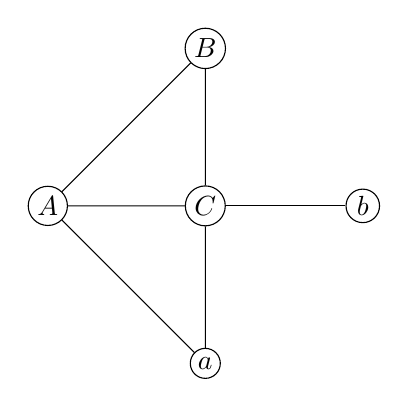
\begin{tikzpicture}[scale=1,every node/.style={draw,circle, inner sep=.05 cm}]
		% \foreach \i in {0,1}{
		% 	\node (\i1) at (\i-1,\i){$A_{\i}$};
		% 	% \node (\i0) at (\i,-1){$h_{\i}$};
		% 	}
		\node (01) at (-1,0){$A$};
		\node (11) at (1,2){$B$};
		\node (02) at (1,0){$C$};
		\node (0-1) at (1,-2){$a$};
		\node (03) at (3,0){$b$};
		\draw (02)--(01)--(11)--(02)--(0-1)--(01);
		\draw (02)--(03);
		% \draw (01)--(11)--(00)--(01);
		\end{tikzpicture}\]
% 	% https://q.uiver.app/#q=WzAsNixbMCwxLCJBIFxcYnVsbGV0Il0sWzEsMSwiQ1xcYnVsbGV0Il0sWzIsMSwiYlxcYnVsbGV0Il0sWzEsMiwiYVxcYnVsbGV0Il0sWzEsMCwiQlxcYnVsbGV0Il0sWzEsMywiRyJdLFswLDEsIiIsMCx7InN0eWxlIjp7ImhlYWQiOnsibmFtZSI6Im5vbmUifX19XSxbMSwyLCIiLDAseyJzdHlsZSI6eyJoZWFkIjp7Im5hbWUiOiJub25lIn19fV0sWzEsMywiIiwwLHsic3R5bGUiOnsiaGVhZCI6eyJuYW1lIjoibm9uZSJ9fX1dLFswLDMsIiIsMix7InN0eWxlIjp7ImhlYWQiOnsibmFtZSI6Im5vbmUifX19XSxbMSw0LCIiLDIseyJzdHlsZSI6eyJoZWFkIjp7Im5hbWUiOiJub25lIn19fV0sWzQsMCwiIiwyLHsic3R5bGUiOnsiaGVhZCI6eyJuYW1lIjoibm9uZSJ9fX1dXQ==
% \[\begin{tikzcd}
% 	& B\bullet \\
% 	{A \bullet} & C\bullet & b\bullet \\
% 	& a\bullet \\
% 	& G
% 	\arrow[no head, from=2-1, to=2-2]
% 	\arrow[no head, from=2-2, to=2-3]
% 	\arrow[no head, from=2-2, to=3-2]
% 	\arrow[no head, from=2-1, to=3-2]
% 	\arrow[no head, from=2-2, to=1-2]
% 	\arrow[no head, from=1-2, to=2-1]
% \end{tikzcd}\]
We label each vertex in $G$ by degree.
\[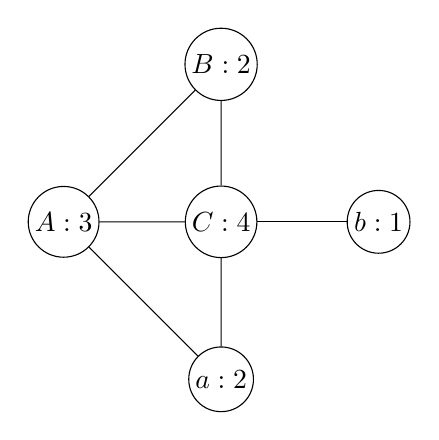
\begin{tikzpicture}[scale=1,every node/.style={draw,circle, inner sep=.05 cm}]
	% \foreach \i in {0,1}{
	% 	\node (\i1) at (\i-1,\i){$A_{\i}$};
	% 	% \node (\i0) at (\i,-1){$h_{\i}$};
	% 	}
	\node (01) at (-1,0){$A:3$};
	\node (11) at (1,2){$B:2$};
	\node (02) at (1,0){$C:4$};
	\node (0-1) at (1,-2){$a:2$};
	\node (03) at (3,0){$b:1$};
	\draw (02)--(01)--(11)--(02)--(0-1)--(01);
	\draw (02)--(03);
	% \draw (01)--(11)--(00)--(01);
	\end{tikzpicture}\]
Our partition of $V$ is $P = \{l_1,l_2,l_3,l_4\}$ where $l_1=\{b\}$, $l_2=\{a,B\}$, $l_3=\{A\}$, and $l_4=\{C\}$. As an example, note $N(A)=\{B,C,a\}$. Therefore, $A$ has two neighbors in $l_2$, namely, $a$ and $B$, and one neighbor in $l_4$, $C$. Thus, $cv(A)=(3,0,2,0,1)$. The reader is encouraged to construct the characterstic vectors for the remaining vertices. To check your work, the results are shown in the table below.
\begin{center}
% \begin{multicols}{2}
	\begin{tabular}{|c|c|c|c|c|c|}
		\hline
		vertices&A&B&C&a&b\\
		\hline
		cv&(3,0,2,0,1)&($2$,0,0,1,1)&($4$,1,2,1,0)&($2$,0,0,1,1)&($2$,0,0,0,1)\\
		\hline
	\end{tabular}\\
% \end{multicols}
\end{center}
\paragraph{}The last step of an iteration is to order the vectors lexicographically. We assign a new label to each vertex based on this ordering. Since 5 is the next integer after our initial 4 classes, first vertex in the order receives a new label of 5. Continue until every vertex has been relabelled. For example, vertex $b$ with characteristic vector $(2,0,0,0,1)$ receives a new label of 5. The result of applying this ordering and relabelling process to the vertices and characteristic vectors of this example is shown in the table and graph below.
\begin{center}
	% \begin{multicols}{2}
		\begin{tabular}{|c|c|c|c|c|c|}
			\hline
			vertices&A&B&C&a&b\\
			\hline
			cv&(3,0,2,0,1)&($2$,0,0,1,1)&($4$,1,2,1,0)&($2$,0,0,1,1)&($2$,0,0,0,1)\\
			\hline
			new label&7&6&8&6&5\\
			\hline
		\end{tabular}
	% \end{multicols}
	\end{center}
	\[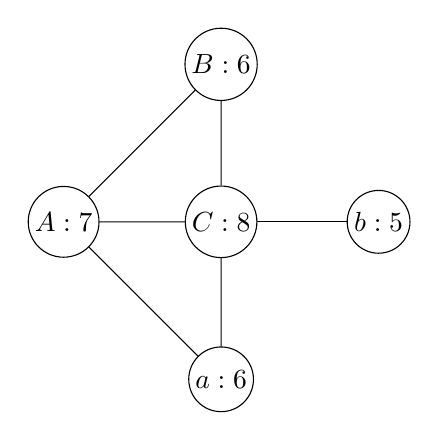
\begin{tikzpicture}[scale=1,every node/.style={draw,circle, inner sep=.05 cm}]
		% \foreach \i in {0,1}{
		% 	\node (\i1) at (\i-1,\i){$A_{\i}$};
		% 	% \node (\i0) at (\i,-1){$h_{\i}$};
		% 	}
		\node (01) at (-1,0){$A:7$};
		\node (11) at (1,2){$B:6$};
		\node (02) at (1,0){$C:8$};
		\node (0-1) at (1,-2){$a:6$};
		\node (03) at (3,0){$b:5$};
		\draw (02)--(01)--(11)--(02)--(0-1)--(01);
		\draw (02)--(03);
		% \draw (01)--(11)--(00)--(01);
		\end{tikzpicture}\]
	% Note that each vertex has a unique label. That is, there are no incomparable vertices, which means we have produced a canonical labeling of $V$.
\end{example}
	\paragraph{} We formalize the steps in the following algorithm.
	\begin{align*}
		&\textbf{WL}\\
	\textbf{Input:}&\;G=\{V,E\}\\
	\textbf{Initialize:}&\text{ Label vertices using degree}\\
	\textbf{Iterate:}&\text{ Produce characteristic vectors, order lexicographically and relabel}\\
	\textbf{Output:}&\text{ Graph }G \text{ with a canonical labelling of the vertex set }
	\end{align*}
	While it is likely clear that comparable vertices (those with different labels) in the output of WL are different, if two vertices $u$ and $v$ end up with the same label, it is not obvious that there exists an automorphism sending $u$ to $v$. However, this non-trivial result is shown in \cite{weisfeiler1968}. Hence, we can be sure that WL results in a canonical labelling for any simple graph.
	
	\begin{remark}
		In \cite{weisfeiler1968}, it is shown that WL will produce a canonical labelling for graphs with loops and/or multiple edges, not just simple graphs.
	\end{remark}The following example applies WL Canonical Labeling until a canonical labelling is produced.
	\begin{example}
        Given the graph $G$ below, we follow WL canonical labelling until the classes stabilize.\\
			\textbf{Input:}% https://q.uiver.app/?q=WzAsNSxbMCwwLCJcXGJ1bGxldCJdLFswLDEsIlxcYnVsbGV0Il0sWzEsMSwiXFxidWxsZXQiXSxbMiwxLCJcXGJ1bGxldCJdLFsxLDAsIlxcYnVsbGV0Il0sWzAsMSwiIiwwLHsic3R5bGUiOnsiaGVhZCI6eyJuYW1lIjoibm9uZSJ9fX1dLFsxLDIsIiIsMCx7InN0eWxlIjp7ImhlYWQiOnsibmFtZSI6Im5vbmUifX19XSxbMiwzLCIiLDAseyJzdHlsZSI6eyJoZWFkIjp7Im5hbWUiOiJub25lIn19fV0sWzEsNCwiIiwwLHsic3R5bGUiOnsiaGVhZCI6eyJuYW1lIjoibm9uZSJ9fX1dXQ==
    \[\begin{tikzcd}
	a\;\bullet & b\;\bullet \\
	c\;\bullet & d\;\bullet & e\;\bullet
	\arrow[no head, from=1-1, to=2-1]
	\arrow[no head, from=2-1, to=2-2]
	\arrow[no head, from=2-2, to=2-3]
	\arrow[no head, from=2-1, to=1-2]
\end{tikzcd}\]
Ordering the vertices of $G$ alphabetically, the adjaceny matrix of $G$ is as follows.
\[A(G)=\bordermatrix{
	&a&b&c&d&e\cr
	a&0&0&1&0&0\cr
	b&0&0&1&0&0\cr
	c&1&1&0&1&0\cr
	d&0&0&1&0&1\cr
	e&0&0&0&1&0
}\]
\textbf{I. Initialize:}
\begin{multicols}{2}
\begin{tabular}{|c|c|}
	\hline
	classes&label\\
	\hline
	\{c\}&3\\
	\{d\}&2\\
	\{a,b,e\}&1\\
	\hline
\end{tabular}\\
\[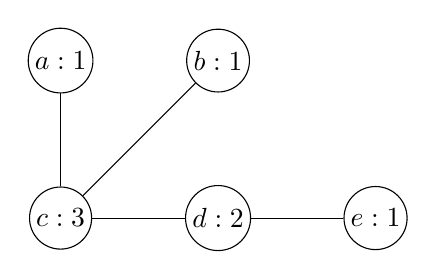
\begin{tikzpicture}[scale=1,every node/.style={draw,circle, inner sep=.05 cm}]
	% \foreach \i in {0,1}{
	% 	\node (\i1) at (\i-1,\i){$A_{\i}$};
	% 	% \node (\i0) at (\i,-1){$h_{\i}$};
	% 	}
	\node (01) at (-1,0){$c:3$};
	\node (11) at (-1,2){$a:1$};
	\node (02) at (1,2){$b:1$};
	\node (0-1) at (1,0){$d:2$};
	\node (03) at (3,0){$e:1$};
	\draw (11)--(01)--(0-1);
	\draw (01)--(02);
	\draw (0-1)--(03);
	% \draw (01)--(11)--(00)--(01);
	\end{tikzpicture}\]
% % https://q.uiver.app/?q=WzAsNSxbMCwwLCIxXFxidWxsZXQiXSxbMCwxLCIzXFxidWxsZXQiXSxbMSwxLCIyXFxidWxsZXQiXSxbMiwxLCIxXFxidWxsZXQiXSxbMSwwLCIxXFxidWxsZXQiXSxbMCwxLCIiLDAseyJzdHlsZSI6eyJoZWFkIjp7Im5hbWUiOiJub25lIn19fV0sWzEsMiwiIiwwLHsic3R5bGUiOnsiaGVhZCI6eyJuYW1lIjoibm9uZSJ9fX1dLFsyLDMsIiIsMCx7InN0eWxlIjp7ImhlYWQiOnsibmFtZSI6Im5vbmUifX19XSxbMSw0LCIiLDAseyJzdHlsZSI6eyJoZWFkIjp7Im5hbWUiOiJub25lIn19fV1d
% \[\begin{tikzcd}
% 	1\bullet & 1\bullet \\
% 	3\bullet & 2\bullet & 1\bullet
% 	\arrow[no head, from=1-1, to=2-1]
% 	\arrow[no head, from=2-1, to=2-2]
% 	\arrow[no head, from=2-2, to=2-3]
% 	\arrow[no head, from=2-1, to=1-2]
% \end{tikzcd}\]
\end{multicols}
\textbf{II. Generate Characteristic Vectors \& Relabel:}\\
\begin{multicols}{2}
\begin{tabular}{|c|c|c|}
	\hline
	classes&cv&relabel\\
	\hline
	\{c\}&(3,2,1,0)&7\\
	\{d\}&(2,1,0,1)&6\\
	\{e\}&(1,0,1,0)&5\\
	\{a,b\}&(1,0,0,1)&4\\
	\hline
\end{tabular}\\
\[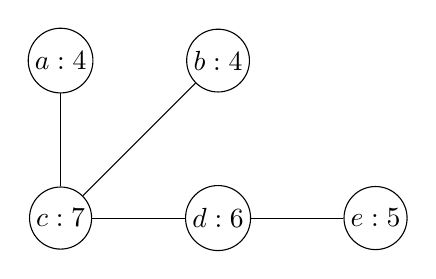
\begin{tikzpicture}[scale=1,every node/.style={draw,circle, inner sep=.05 cm}]
	% \foreach \i in {0,1}{
	% 	\node (\i1) at (\i-1,\i){$A_{\i}$};
	% 	% \node (\i0) at (\i,-1){$h_{\i}$};
	% 	}
	\node (01) at (-1,0){$c:7$};
	\node (11) at (-1,2){$a:4$};
	\node (02) at (1,2){$b:4$};
	\node (0-1) at (1,0){$d:6$};
	\node (03) at (3,0){$e:5$};
	\draw (11)--(01)--(0-1);
	\draw (01)--(02);
	\draw (0-1)--(03);
	% \draw (01)--(11)--(00)--(01);
	\end{tikzpicture}\]
% % https://q.uiver.app/?q=WzAsNSxbMCwwLCIoMSwwLDAsMSlcXGJ1bGxldCJdLFswLDEsIigzLDIsMSwwKVxcYnVsbGV0Il0sWzEsMSwiKDIsMSwwLDEpXFxidWxsZXQiXSxbMiwxLCIoMSwwLDEsMClcXGJ1bGxldCJdLFsxLDAsIigxLDAsMCwxKVxcYnVsbGV0Il0sWzAsMSwiIiwwLHsic3R5bGUiOnsiaGVhZCI6eyJuYW1lIjoibm9uZSJ9fX1dLFsxLDIsIiIsMCx7InN0eWxlIjp7ImhlYWQiOnsibmFtZSI6Im5vbmUifX19XSxbMiwzLCIiLDAseyJzdHlsZSI6eyJoZWFkIjp7Im5hbWUiOiJub25lIn19fV0sWzEsNCwiIiwwLHsic3R5bGUiOnsiaGVhZCI6eyJuYW1lIjoibm9uZSJ9fX1dXQ==
% \[\begin{tikzcd}
% 	{4\;\bullet} & {4\;\bullet} \\
% 	{7\;\bullet} & {6\;\bullet} & {5\;\bullet}
% 	\arrow[no head, from=1-1, to=2-1]
% 	\arrow[no head, from=2-1, to=2-2]
% 	\arrow[no head, from=2-2, to=2-3]
% 	\arrow[no head, from=2-1, to=1-2]
% \end{tikzcd}\]
\end{multicols}\newpage
\textbf{III. Iterate:} \\
Since the classes stay the same, the process terminates here. 
\begin{multicols}{2}
\begin{tabular}{|c|c|}
	\hline
	classes&cv\\
	\hline
	\{c\}&(7,2,0,1,0)\\
	\{d\}&(6,0,1,0,1)\\
	\{e\}&(5,0,0,1,0)\\
	\{a,b\}&(4,0,0,1,0)\\
	\hline
\end{tabular}\\
\[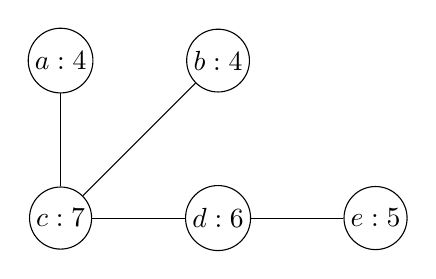
\begin{tikzpicture}[scale=1,every node/.style={draw,circle, inner sep=.05 cm}]
	% \foreach \i in {0,1}{
	% 	\node (\i1) at (\i-1,\i){$A_{\i}$};
	% 	% \node (\i0) at (\i,-1){$h_{\i}$};
	% 	}
	\node (01) at (-1,0){$c:7$};
	\node (11) at (-1,2){$a:4$};
	\node (02) at (1,2){$b:4$};
	\node (0-1) at (1,0){$d:6$};
	\node (03) at (3,0){$e:5$};
	\draw (11)--(01)--(0-1);
	\draw (01)--(02);
	\draw (0-1)--(03);
	% \draw (01)--(11)--(00)--(01);
	\end{tikzpicture}\]
% % https://q.uiver.app/?q=WzAsNSxbMCwwLCIoMSwwLDAsMSlcXGJ1bGxldCJdLFswLDEsIigzLDIsMSwwKVxcYnVsbGV0Il0sWzEsMSwiKDIsMSwwLDEpXFxidWxsZXQiXSxbMiwxLCIoMSwwLDEsMClcXGJ1bGxldCJdLFsxLDAsIigxLDAsMCwxKVxcYnVsbGV0Il0sWzAsMSwiIiwwLHsic3R5bGUiOnsiaGVhZCI6eyJuYW1lIjoibm9uZSJ9fX1dLFsxLDIsIiIsMCx7InN0eWxlIjp7ImhlYWQiOnsibmFtZSI6Im5vbmUifX19XSxbMiwzLCIiLDAseyJzdHlsZSI6eyJoZWFkIjp7Im5hbWUiOiJub25lIn19fV0sWzEsNCwiIiwwLHsic3R5bGUiOnsiaGVhZCI6eyJuYW1lIjoibm9uZSJ9fX1dXQ==
% \[\begin{tikzcd}
% 	{4\;\bullet} & {4\;\bullet} \\
% 	{7\;\bullet} & {6\;\bullet} & {5\;\bullet}
% 	\arrow[no head, from=1-1, to=2-1]
% 	\arrow[no head, from=2-1, to=2-2]
% 	\arrow[no head, from=2-2, to=2-3]
% 	\arrow[no head, from=2-1, to=1-2]
% \end{tikzcd}\]
\end{multicols}
The following is a canonical form of $G$ generated by WL.
\[Canon(G)=\bordermatrix{
	&a&b&e&d&c\cr
	a&0&0&0&0&1\cr
	b&0&0&0&0&1\cr
	e&0&0&0&1&0\cr
	d&0&0&1&0&1\cr
	c&1&1&0&1&0
}\]
% \[Canon(G)=\begin{pmatrix}
% 	0&0&0&0&1\\
% 	0&0&0&0&1\\
% 	0&0&0&1&0\\
% 	0&0&1&0&1\\
% 	1&1&0&1&0
% \end{pmatrix}\]
% Using $Canon(G)$, we generate a graph labelled using the first entry of each characteristic vector. 
% % https://q.uiver.app/?q=WzAsNSxbMCwwLCIxXFxidWxsZXQiXSxbMCwxLCI0XFxidWxsZXQiXSxbMSwxLCIzXFxidWxsZXQiXSxbMiwxLCIyXFxidWxsZXQiXSxbMSwwLCIxXFxidWxsZXQiXSxbMCwxLCIiLDAseyJzdHlsZSI6eyJoZWFkIjp7Im5hbWUiOiJub25lIn19fV0sWzEsMiwiIiwwLHsic3R5bGUiOnsiaGVhZCI6eyJuYW1lIjoibm9uZSJ9fX1dLFsyLDMsIiIsMCx7InN0eWxlIjp7ImhlYWQiOnsibmFtZSI6Im5vbmUifX19XSxbMSw0LCIiLDAseyJzdHlsZSI6eyJoZWFkIjp7Im5hbWUiOiJub25lIn19fV1d
% \[\begin{tikzcd}
% 	4\bullet & 4\bullet \\
% 	7\bullet & 6\bullet & 5\bullet
% 	\arrow[no head, from=1-1, to=2-1]
% 	\arrow[no head, from=2-1, to=2-2]
% 	\arrow[no head, from=2-2, to=2-3]
% 	\arrow[no head, from=2-1, to=1-2]
% \end{tikzcd}\]

	





   
Notice that $a$ and $b$ are in the same class, that is, $a$ and $b$ are incomparable. Since the relevant result from \cite{weisfeiler1968} mentioned above, ensures that this is a canonical form of $G$. Hence, there exist a graph automorphism sending $a$ to $b$. The function, $f:\{a,b,c,d,e\}\rightarrow\{a,b,c,d,e\}$, defined by \[f(u)=\begin{cases}
	b,\;u=a\\
	a,\;u=b\\
	u,\;u\ne a,b
\end{cases}\]is such a function.
% If two vertices $u,v\in V$ are in the same class when the algorithm terminates, then there exists an automorphism sending $u$ to $v$ \cite{weisfeiler1968}. Thus, the partial ordering of $V$ given by such classes is a canonical form by Definition 2.7.
% On the other hand, if each vertex has a unique class when the algorithm terminates, then the partial ordering of $V$ given by the classes leaves no incomparable vertices. In this case, the ordering on $V$ given by the classes is a canonical form as well, satisfying Definition 2.7 trivially. 
    \end{example} 

	\begin{remark}
		Since WL iteratively produces partitions of vertex sets, it is also called \textit{color refinement}. The color of a vertex is its class at any given iteration. 
	\end{remark}
\subsection{A Non-Isomorphism Test}
As mentioned in the previous subsection, we can use a canonization algorithm to produce a graph identification algorithm. However, unless we add extra machinery, canonization is not sufficient for graph identification. In that case, we can only hope to produce an algorithm that can determine two graphs are not isomorphic. In what follows, we present such an algorithm based on WL, the \textit{WL Non-Isomorphism Test}, adopted from \cite{shervashidze2011weisfeiler}. This test differs from WL in two key ways. First, the input of WL Non-Isomorphism Test is two graphs rather than a single graph.  WL is applied to each graph at the same time, where new vertex labels for both graphs come from same alphabet. Second, at initialization, a label string is generated for each graph $G$, denoted $s(G)$, using the initial labels as follows. The $k^{th}$ entry in a label string for a graph $G$ is the number of vertices of $G$ with label $k$. After each iteration, a new label string is generated based on the new labels, then concatenated to the end of the old string. If the graphs have different strings at any step then the algorithm terminates immediately, returning that the two graphs are not isomorphic. 
		\paragraph{}\begin{align*}
			&\textbf{WL Non-Isomorphism Test }\\
		\textbf{Input:}&\text{ Graphs }G=\{V,E\},\;G'=\{V',E'\}\\
		\textbf{Initialize:}&\text{ Label the vertices using degree}\\
		&\text{Generate and compare label strings}\\
		&\text{If strings are not equal, terminate}\\
		\textbf{Iterate:}&\text{ Produce characteristic vectors for all vertices in }G\text{ and }G'\\
		&\text{ Order characteristic vectors, relabel}\\
		&\text{If classes did not change, terminate}\\
		&\text{Generate new label string }\\
		&\text{If strings are not equal, terminate}\\
		\textbf{Output:}&\text{ A graph isomorphism from $G$ to $G'$ does not exist }\\&\text{or NULL}
		\end{align*}
		\begin{example}
			This example applies the WL Non-Isomorphism Test to $H$ and $H'$.
			\begin{multicols}{2}
				$H$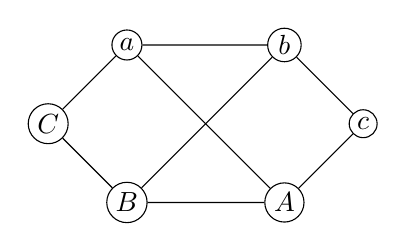
\begin{tikzpicture}[scale=1,every node/.style={draw,circle, inner sep=.05 cm}]
				% \foreach \i in {0,1}{
				% 	\node (\i1) at (\i-1,\i){$A_{\i}$};
				% 	% \node (\i0) at (\i,-1){$h_{\i}$};
				% 	}
				\node (-10) at (-1,0){$C$};
				\node (02) at (0,1){$a$};
				\node (0-2) at (0,-1){$B$};
				\node (32) at (2,1){$b$};
				\node (3-2) at (2,-1){$A$};
				\node (50) at (3,0){$c$};
				\draw (02)--(-10)--(0-2);
				\draw (3-2)--(02)--(32);
				\draw (32)--(0-2)--(3-2);
				\draw (32)--(50)--(3-2);
				% \draw (01)--(11)--(00)--(01);
				\end{tikzpicture}\\
				$H'$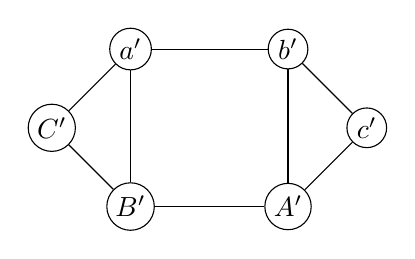
\begin{tikzpicture}[scale=1,every node/.style={draw,circle, inner sep=.05 cm}]
					% \foreach \i in {0,1}{
					% 	\node (\i1) at (\i-1,\i){$A_{\i}$};
					% 	% \node (\i0) at (\i,-1){$h_{\i}$};
					% 	}
					\node (-10) at (-1,0){$C'$};
					\node (02) at (0,1){$a'$};
					\node (0-2) at (0,-1){$B'$};
					\node (32) at (2,1){$b'$};
					\node (3-2) at (2,-1){$A'$};
					\node (50) at (3,0){$c'$};
					\draw (02)--(-10)--(0-2);
					\draw (3-2)--(0-2)--(02)--(32)--(3-2);
					% \draw (0-2)--(3-2);
					\draw (32)--(50)--(3-2);
					% \draw (01)--(11)--(00)--(01);
					\end{tikzpicture}
			\end{multicols}
% 			   % https://q.uiver.app/?q=WzAsMTQsWzIsMCwiXFxidWxsZXQiXSxbMywxLCJcXGJ1bGxldCJdLFsyLDIsIlxcYnVsbGV0Il0sWzEsMiwiXFxidWxsZXQiXSxbMCwxLCJcXGJ1bGxldCJdLFsxLDAsIlxcYnVsbGV0Il0sWzcsMCwiXFxidWxsZXQiXSxbOCwxLCJcXGJ1bGxldCJdLFs3LDIsIlxcYnVsbGV0Il0sWzYsMiwiXFxidWxsZXQiXSxbNSwxLCJcXGJ1bGxldCJdLFs2LDAsIlxcYnVsbGV0Il0sWzEsMywiSCJdLFs3LDMsIkgnIl0sWzAsMSwiIiwwLHsic3R5bGUiOnsiaGVhZCI6eyJuYW1lIjoibm9uZSJ9fX1dLFsxLDIsIiIsMCx7InN0eWxlIjp7ImhlYWQiOnsibmFtZSI6Im5vbmUifX19XSxbMiwzLCIiLDAseyJzdHlsZSI6eyJoZWFkIjp7Im5hbWUiOiJub25lIn19fV0sWzMsNCwiIiwwLHsic3R5bGUiOnsiaGVhZCI6eyJuYW1lIjoibm9uZSJ9fX1dLFs0LDUsIiIsMCx7InN0eWxlIjp7ImhlYWQiOnsibmFtZSI6Im5vbmUifX19XSxbNiw3LCIiLDAseyJzdHlsZSI6eyJoZWFkIjp7Im5hbWUiOiJub25lIn19fV0sWzcsOCwiIiwwLHsic3R5bGUiOnsiaGVhZCI6eyJuYW1lIjoibm9uZSJ9fX1dLFs4LDksIiIsMCx7InN0eWxlIjp7ImhlYWQiOnsibmFtZSI6Im5vbmUifX19XSxbOSwxMCwiIiwwLHsic3R5bGUiOnsiaGVhZCI6eyJuYW1lIjoibm9uZSJ9fX1dLFsxMCwxMSwiIiwwLHsic3R5bGUiOnsiaGVhZCI6eyJuYW1lIjoibm9uZSJ9fX1dLFsxMSw2LCIiLDAseyJzdHlsZSI6eyJoZWFkIjp7Im5hbWUiOiJub25lIn19fV0sWzExLDksIiIsMSx7InN0eWxlIjp7ImhlYWQiOnsibmFtZSI6Im5vbmUifX19XSxbNiw4LCIiLDEseyJzdHlsZSI6eyJoZWFkIjp7Im5hbWUiOiJub25lIn19fV0sWzUsMCwiIiwxLHsic3R5bGUiOnsiaGVhZCI6eyJuYW1lIjoibm9uZSJ9fX1dLFszLDAsIiIsMSx7InN0eWxlIjp7ImhlYWQiOnsibmFtZSI6Im5vbmUifX19XSxbNSwyLCIiLDEseyJzdHlsZSI6eyJoZWFkIjp7Im5hbWUiOiJub25lIn19fV1d
% \[\begin{tikzcd}[ampersand replacement=\&]
% 	\& a\;\bullet \& b\;\bullet \&\&\&\& a'\;\bullet \& b'\;\bullet \\
% 	C\;\bullet \&\&\& c\;\bullet \&\& C'\;\bullet \&\&\& c'\;\bullet \\
% 	\& B\;\;\bullet \& A\;\bullet \&\&\&\& B'\;\bullet \& A'\;\bullet \\
% 	\& H \&\&\&\&\&\& {H'}
% 	\arrow[no head, from=1-3, to=2-4]
% 	\arrow[no head, from=2-4, to=3-3]
% 	\arrow[no head, from=3-3, to=3-2]
% 	\arrow[no head, from=3-2, to=2-1]
% 	\arrow[no head, from=2-1, to=1-2]
% 	\arrow[no head, from=1-8, to=2-9]
% 	\arrow[no head, from=2-9, to=3-8]
% 	\arrow[no head, from=3-8, to=3-7]
% 	\arrow[no head, from=3-7, to=2-6]
% 	\arrow[no head, from=2-6, to=1-7]
% 	\arrow[no head, from=1-7, to=1-8]
% 	\arrow[no head, from=1-7, to=3-7]
% 	\arrow[no head, from=1-8, to=3-8]
% 	\arrow[no head, from=1-2, to=1-3]
% 	\arrow[no head, from=3-2, to=1-3]
% 	\arrow[no head, from=1-2, to=3-3]
% \end{tikzcd}\]
\newpage
\textbf{I. Initialize:} Label the vertices by their degree and construct label strings.
\begin{multicols}{2}
	$H$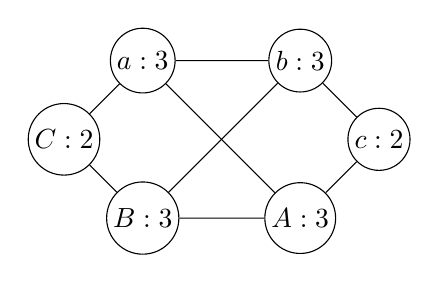
\begin{tikzpicture}[scale=1,every node/.style={draw,circle, inner sep=.05 cm}]
	% \foreach \i in {0,1}{
	% 	\node (\i1) at (\i-1,\i){$A_{\i}$};
	% 	% \node (\i0) at (\i,-1){$h_{\i}$};
	% 	}
	\node (-10) at (-1,0){$C:2$};
	\node (02) at (0,1){$a:3$};
	\node (0-2) at (0,-1){$B:3$};
	\node (32) at (2,1){$b:3$};
	\node (3-2) at (2,-1){$A:3$};
	\node (50) at (3,0){$c:2$};
	\draw (02)--(-10)--(0-2);
	\draw (3-2)--(02)--(32);
	\draw (32)--(0-2)--(3-2);
	\draw (32)--(50)--(3-2);
	% \draw (01)--(11)--(00)--(01);
	\end{tikzpicture}\\
	$H'$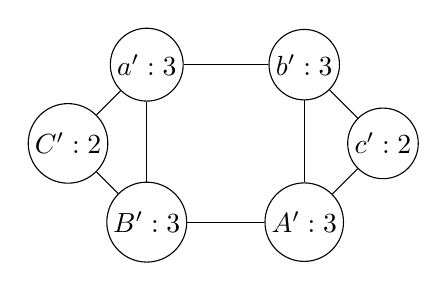
\begin{tikzpicture}[scale=1,every node/.style={draw,circle, inner sep=.05 cm}]
		% \foreach \i in {0,1}{
		% 	\node (\i1) at (\i-1,\i){$A_{\i}$};
		% 	% \node (\i0) at (\i,-1){$h_{\i}$};
		% 	}
		\node (-10) at (-1,0){$C':2$};
		\node (02) at (0,1){$a':3$};
		\node (0-2) at (0,-1){$B':3$};
		\node (32) at (2,1){$b':3$};
		\node (3-2) at (2,-1){$A':3$};
		\node (50) at (3,0){$c':2$};
		\draw (02)--(-10)--(0-2);
		\draw (3-2)--(0-2)--(02)--(32)--(3-2);
		% \draw (0-2)--(3-2);
		\draw (32)--(50)--(3-2);
		% \draw (01)--(11)--(00)--(01);
		\end{tikzpicture}
\end{multicols}
% % https://q.uiver.app/?q=WzAsMTIsWzIsMCwiMyJdLFszLDEsIjIiXSxbMiwyLCIzIl0sWzEsMiwiMyJdLFswLDEsIjIiXSxbMSwwLCIzIl0sWzcsMCwiMyJdLFs4LDEsIjIiXSxbNywyLCIzIl0sWzYsMiwiMyJdLFs1LDEsIjIiXSxbNiwwLCIzIl0sWzAsMSwiIiwwLHsic3R5bGUiOnsiaGVhZCI6eyJuYW1lIjoibm9uZSJ9fX1dLFsxLDIsIiIsMCx7InN0eWxlIjp7ImhlYWQiOnsibmFtZSI6Im5vbmUifX19XSxbMiwzLCIiLDAseyJzdHlsZSI6eyJoZWFkIjp7Im5hbWUiOiJub25lIn19fV0sWzMsNCwiIiwwLHsic3R5bGUiOnsiaGVhZCI6eyJuYW1lIjoibm9uZSJ9fX1dLFs0LDUsIiIsMCx7InN0eWxlIjp7ImhlYWQiOnsibmFtZSI6Im5vbmUifX19XSxbNiw3LCIiLDAseyJzdHlsZSI6eyJoZWFkIjp7Im5hbWUiOiJub25lIn19fV0sWzcsOCwiIiwwLHsic3R5bGUiOnsiaGVhZCI6eyJuYW1lIjoibm9uZSJ9fX1dLFs4LDksIiIsMCx7InN0eWxlIjp7ImhlYWQiOnsibmFtZSI6Im5vbmUifX19XSxbOSwxMCwiIiwwLHsic3R5bGUiOnsiaGVhZCI6eyJuYW1lIjoibm9uZSJ9fX1dLFsxMCwxMSwiIiwwLHsic3R5bGUiOnsiaGVhZCI6eyJuYW1lIjoibm9uZSJ9fX1dLFsxMSw2LCIiLDAseyJzdHlsZSI6eyJoZWFkIjp7Im5hbWUiOiJub25lIn19fV0sWzExLDksIiIsMSx7InN0eWxlIjp7ImhlYWQiOnsibmFtZSI6Im5vbmUifX19XSxbNiw4LCIiLDEseyJzdHlsZSI6eyJoZWFkIjp7Im5hbWUiOiJub25lIn19fV0sWzUsMCwiIiwxLHsic3R5bGUiOnsiaGVhZCI6eyJuYW1lIjoibm9uZSJ9fX1dLFszLDAsIiIsMSx7InN0eWxlIjp7ImhlYWQiOnsibmFtZSI6Im5vbmUifX19XSxbNSwyLCIiLDEseyJzdHlsZSI6eyJoZWFkIjp7Im5hbWUiOiJub25lIn19fV1d
% \[\begin{tikzcd}[ampersand replacement=\&]
% 	\& 3 \& 3 \&\&\&\& 3 \& 3 \\
% 	2 \&\&\& 2 \&\& 2 \&\&\& 2 \\
% 	\& 3 \& 3 \&\&\&\& 3 \& 3
% 	\arrow[no head, from=1-3, to=2-4]
% 	\arrow[no head, from=2-4, to=3-3]
% 	\arrow[no head, from=3-3, to=3-2]
% 	\arrow[no head, from=3-2, to=2-1]
% 	\arrow[no head, from=2-1, to=1-2]
% 	\arrow[no head, from=1-8, to=2-9]
% 	\arrow[no head, from=2-9, to=3-8]
% 	\arrow[no head, from=3-8, to=3-7]
% 	\arrow[no head, from=3-7, to=2-6]
% 	\arrow[no head, from=2-6, to=1-7]
% 	\arrow[no head, from=1-7, to=1-8]
% 	\arrow[no head, from=1-7, to=3-7]
% 	\arrow[no head, from=1-8, to=3-8]
% 	\arrow[no head, from=1-2, to=1-3]
% 	\arrow[no head, from=3-2, to=1-3]
% 	\arrow[no head, from=1-2, to=3-3]
% \end{tikzcd}\]
\begin{multicols}{2}
\begin{tabular}{|c|c|}
	\hline
	classes&label\\
	\hline
	\{a,b,A,B\}&3\\
	\{c,C\}&2\\
	\{\}&1\\
	\hline
\end{tabular}
$s(H) = (024)$ \\

\begin{tabular}{|c|c|}
	\hline
	classes&label\\
	\hline
	\{a',b',A',B'\}&3\\
	\{c',C'\}&2\\
	\{\}&1\\
	\hline
\end{tabular}
$s(H') = (024)$
\end{multicols}
\textbf{II. Generate Characteristic Vectors \& Relabel:}\\
Notice that the labels do not change from the previous step, so the process terminates after relabelling.
\begin{multicols}{2}
\begin{tabular}{|c|c|c|}
	\hline
	classes&cv&label\\
	\hline
	\{a,b,A,B\}&(3,0,1,2)&5\\
	\{c,C\}&(2,0,0,2)&4\\
	\{\}&&\\
	\hline
\end{tabular}

\begin{tabular}{|c|c|c|}
	\hline
	classes&cv&label\\
	\hline
	\{a',b',A',B'\}&(3,0,1,2)&5\\
	\{c',C'\}&(2,0,0,2)&4\\
	\{\}&&\\
	\hline
\end{tabular}
\end{multicols}

% Next, produce characteristic vectors.
% % https://q.uiver.app/?q=WzAsMTIsWzIsMCwiKDMsMCwxLDIpIl0sWzMsMSwiKDIsMCwwLDIpIl0sWzIsMiwiKDMsMCwxLDIpIl0sWzEsMiwiKDMsMCwxLDIpIl0sWzAsMSwiKDIsMCwwLDIpIl0sWzEsMCwiKDMsMCwxLDIpIl0sWzIsMywiKDMsMCwxLDIpIl0sWzMsNCwiKDIsMCwwLDIpIl0sWzIsNSwiKDMsMCwxLDIpIl0sWzEsNSwiKDMsMCwxLDIpIl0sWzAsNCwiKDIsMCwwLDIpIl0sWzEsMywiKDMsMCwxLDIpIl0sWzAsMSwiIiwwLHsic3R5bGUiOnsiaGVhZCI6eyJuYW1lIjoibm9uZSJ9fX1dLFsxLDIsIiIsMCx7InN0eWxlIjp7ImhlYWQiOnsibmFtZSI6Im5vbmUifX19XSxbMiwzLCIiLDAseyJzdHlsZSI6eyJoZWFkIjp7Im5hbWUiOiJub25lIn19fV0sWzMsNCwiIiwwLHsic3R5bGUiOnsiaGVhZCI6eyJuYW1lIjoibm9uZSJ9fX1dLFs0LDUsIiIsMCx7InN0eWxlIjp7ImhlYWQiOnsibmFtZSI6Im5vbmUifX19XSxbNiw3LCIiLDAseyJzdHlsZSI6eyJoZWFkIjp7Im5hbWUiOiJub25lIn19fV0sWzcsOCwiIiwwLHsic3R5bGUiOnsiaGVhZCI6eyJuYW1lIjoibm9uZSJ9fX1dLFs4LDksIiIsMCx7InN0eWxlIjp7ImhlYWQiOnsibmFtZSI6Im5vbmUifX19XSxbOSwxMCwiIiwwLHsic3R5bGUiOnsiaGVhZCI6eyJuYW1lIjoibm9uZSJ9fX1dLFsxMCwxMSwiIiwwLHsic3R5bGUiOnsiaGVhZCI6eyJuYW1lIjoibm9uZSJ9fX1dLFsxMSw2LCIiLDAseyJzdHlsZSI6eyJoZWFkIjp7Im5hbWUiOiJub25lIn19fV0sWzExLDksIiIsMSx7InN0eWxlIjp7ImhlYWQiOnsibmFtZSI6Im5vbmUifX19XSxbNiw4LCIiLDEseyJzdHlsZSI6eyJoZWFkIjp7Im5hbWUiOiJub25lIn19fV0sWzUsMCwiIiwxLHsic3R5bGUiOnsiaGVhZCI6eyJuYW1lIjoibm9uZSJ9fX1dLFszLDAsIiIsMSx7InN0eWxlIjp7ImhlYWQiOnsibmFtZSI6Im5vbmUifX19XSxbNSwyLCIiLDEseyJzdHlsZSI6eyJoZWFkIjp7Im5hbWUiOiJub25lIn19fV1d
% \[\begin{tikzcd}[ampersand replacement=\&]
% 	\& {(3,0,1,2)} \& {(3,0,1,2)} \\
% 	{(2,0,0,2)} \&\&\& {(2,0,0,2)} \\
% 	\& {(3,0,1,2)} \& {(3,0,1,2)} \\
% 	\& {(3,0,1,2)} \& {(3,0,1,2)} \\
% 	{(2,0,0,2)} \&\&\& {(2,0,0,2)} \\
% 	\& {(3,0,1,2)} \& {(3,0,1,2)}
% 	\arrow[no head, from=1-3, to=2-4]
% 	\arrow[no head, from=2-4, to=3-3]
% 	\arrow[no head, from=3-3, to=3-2]
% 	\arrow[no head, from=3-2, to=2-1]
% 	\arrow[no head, from=2-1, to=1-2]
% 	\arrow[no head, from=4-3, to=5-4]
% 	\arrow[no head, from=5-4, to=6-3]
% 	\arrow[no head, from=6-3, to=6-2]
% 	\arrow[no head, from=6-2, to=5-1]
% 	\arrow[no head, from=5-1, to=4-2]
% 	\arrow[no head, from=4-2, to=4-3]
% 	\arrow[no head, from=4-2, to=6-2]
% 	\arrow[no head, from=4-3, to=6-3]
% 	\arrow[no head, from=1-2, to=1-3]
% 	\arrow[no head, from=3-2, to=1-3]
% 	\arrow[no head, from=1-2, to=3-3]
% \end{tikzcd}\]
% Order the vectors and relabel.
% % https://q.uiver.app/?q=WzAsMTIsWzIsMCwiMiJdLFszLDEsIjEiXSxbMiwyLCIyIl0sWzEsMiwiMiJdLFswLDEsIjEiXSxbMSwwLCIyIl0sWzIsMywiMiJdLFszLDQsIjEiXSxbMiw1LCIyIl0sWzEsNSwiMiJdLFswLDQsIjEiXSxbMSwzLCIyIl0sWzAsMSwiIiwwLHsic3R5bGUiOnsiaGVhZCI6eyJuYW1lIjoibm9uZSJ9fX1dLFsxLDIsIiIsMCx7InN0eWxlIjp7ImhlYWQiOnsibmFtZSI6Im5vbmUifX19XSxbMiwzLCIiLDAseyJzdHlsZSI6eyJoZWFkIjp7Im5hbWUiOiJub25lIn19fV0sWzMsNCwiIiwwLHsic3R5bGUiOnsiaGVhZCI6eyJuYW1lIjoibm9uZSJ9fX1dLFs0LDUsIiIsMCx7InN0eWxlIjp7ImhlYWQiOnsibmFtZSI6Im5vbmUifX19XSxbNiw3LCIiLDAseyJzdHlsZSI6eyJoZWFkIjp7Im5hbWUiOiJub25lIn19fV0sWzcsOCwiIiwwLHsic3R5bGUiOnsiaGVhZCI6eyJuYW1lIjoibm9uZSJ9fX1dLFs4LDksIiIsMCx7InN0eWxlIjp7ImhlYWQiOnsibmFtZSI6Im5vbmUifX19XSxbOSwxMCwiIiwwLHsic3R5bGUiOnsiaGVhZCI6eyJuYW1lIjoibm9uZSJ9fX1dLFsxMCwxMSwiIiwwLHsic3R5bGUiOnsiaGVhZCI6eyJuYW1lIjoibm9uZSJ9fX1dLFsxMSw2LCIiLDAseyJzdHlsZSI6eyJoZWFkIjp7Im5hbWUiOiJub25lIn19fV0sWzExLDksIiIsMSx7InN0eWxlIjp7ImhlYWQiOnsibmFtZSI6Im5vbmUifX19XSxbNiw4LCIiLDEseyJzdHlsZSI6eyJoZWFkIjp7Im5hbWUiOiJub25lIn19fV0sWzUsMCwiIiwxLHsic3R5bGUiOnsiaGVhZCI6eyJuYW1lIjoibm9uZSJ9fX1dLFszLDAsIiIsMSx7InN0eWxlIjp7ImhlYWQiOnsibmFtZSI6Im5vbmUifX19XSxbNSwyLCIiLDEseyJzdHlsZSI6eyJoZWFkIjp7Im5hbWUiOiJub25lIn19fV1d
% \[\begin{tikzcd}[ampersand replacement=\&]
% 	\& 2 \& 2 \\
% 	1 \&\&\& 1 \\
% 	\& 2 \& 2 \\
% 	\& 2 \& 2 \\
% 	1 \&\&\& 1 \\
% 	\& 2 \& 2
% 	\arrow[no head, from=1-3, to=2-4]
% 	\arrow[no head, from=2-4, to=3-3]
% 	\arrow[no head, from=3-3, to=3-2]
% 	\arrow[no head, from=3-2, to=2-1]
% 	\arrow[no head, from=2-1, to=1-2]
% 	\arrow[no head, from=4-3, to=5-4]
% 	\arrow[no head, from=5-4, to=6-3]
% 	\arrow[no head, from=6-3, to=6-2]
% 	\arrow[no head, from=6-2, to=5-1]
% 	\arrow[no head, from=5-1, to=4-2]
% 	\arrow[no head, from=4-2, to=4-3]
% 	\arrow[no head, from=4-2, to=6-2]
% 	\arrow[no head, from=4-3, to=6-3]
% 	\arrow[no head, from=1-2, to=1-3]
% 	\arrow[no head, from=3-2, to=1-3]
% 	\arrow[no head, from=1-2, to=3-3]
% \end{tikzcd}\]
% Iterate.
% % https://q.uiver.app/?q=WzAsMTIsWzIsMCwiKDIsMSwyKSJdLFszLDEsIigxLDAsMikiXSxbMiwyLCIoMiwxLDIpIl0sWzEsMiwiKDIsMSwyKSJdLFswLDEsIigxLDAsMikiXSxbMSwwLCIoMiwxLDIpIl0sWzIsMywiKDIsMSwyKSJdLFszLDQsIigxLDAsMikiXSxbMiw1LCIoMiwxLDIpIl0sWzAsNCwiKDEsMCwyKSJdLFsxLDMsIigyLDEsMikiXSxbMSw1LCIoMiwxLDIpIl0sWzAsMSwiIiwwLHsic3R5bGUiOnsiaGVhZCI6eyJuYW1lIjoibm9uZSJ9fX1dLFsxLDIsIiIsMCx7InN0eWxlIjp7ImhlYWQiOnsibmFtZSI6Im5vbmUifX19XSxbMiwzLCIiLDAseyJzdHlsZSI6eyJoZWFkIjp7Im5hbWUiOiJub25lIn19fV0sWzMsNCwiIiwwLHsic3R5bGUiOnsiaGVhZCI6eyJuYW1lIjoibm9uZSJ9fX1dLFs0LDUsIiIsMCx7InN0eWxlIjp7ImhlYWQiOnsibmFtZSI6Im5vbmUifX19XSxbNiw3LCIiLDAseyJzdHlsZSI6eyJoZWFkIjp7Im5hbWUiOiJub25lIn19fV0sWzcsOCwiIiwwLHsic3R5bGUiOnsiaGVhZCI6eyJuYW1lIjoibm9uZSJ9fX1dLFs5LDEwLCIiLDAseyJzdHlsZSI6eyJoZWFkIjp7Im5hbWUiOiJub25lIn19fV0sWzEwLDYsIiIsMCx7InN0eWxlIjp7ImhlYWQiOnsibmFtZSI6Im5vbmUifX19XSxbNiw4LCIiLDEseyJzdHlsZSI6eyJoZWFkIjp7Im5hbWUiOiJub25lIn19fV0sWzUsMCwiIiwxLHsic3R5bGUiOnsiaGVhZCI6eyJuYW1lIjoibm9uZSJ9fX1dLFszLDAsIiIsMSx7InN0eWxlIjp7ImhlYWQiOnsibmFtZSI6Im5vbmUifX19XSxbNSwyLCIiLDEseyJzdHlsZSI6eyJoZWFkIjp7Im5hbWUiOiJub25lIn19fV0sWzgsMTEsIiIsMCx7InN0eWxlIjp7ImhlYWQiOnsibmFtZSI6Im5vbmUifX19XSxbMTEsOSwiIiwwLHsic3R5bGUiOnsiaGVhZCI6eyJuYW1lIjoibm9uZSJ9fX1dLFsxMCwxMSwiIiwxLHsic3R5bGUiOnsiaGVhZCI6eyJuYW1lIjoibm9uZSJ9fX1dXQ==
% \[\begin{tikzcd}[ampersand replacement=\&]
% 	\& {(2,1,2)} \& {(2,1,2)} \\
% 	{(1,0,2)} \&\&\& {(1,0,2)} \\
% 	\& {(2,1,2)} \& {(2,1,2)} \\
% 	\& {(2,1,2)} \& {(2,1,2)} \\
% 	{(1,0,2)} \&\&\& {(1,0,2)} \\
% 	\& {(2,1,2)} \& {(2,1,2)}
% 	\arrow[no head, from=1-3, to=2-4]
% 	\arrow[no head, from=2-4, to=3-3]
% 	\arrow[no head, from=3-3, to=3-2]
% 	\arrow[no head, from=3-2, to=2-1]
% 	\arrow[no head, from=2-1, to=1-2]
% 	\arrow[no head, from=4-3, to=5-4]
% 	\arrow[no head, from=5-4, to=6-3]
% 	\arrow[no head, from=5-1, to=4-2]
% 	\arrow[no head, from=4-2, to=4-3]
% 	\arrow[no head, from=4-3, to=6-3]
% 	\arrow[no head, from=1-2, to=1-3]
% 	\arrow[no head, from=3-2, to=1-3]
% 	\arrow[no head, from=1-2, to=3-3]
% 	\arrow[no head, from=6-3, to=6-2]
% 	\arrow[no head, from=6-2, to=5-1]
% 	\arrow[no head, from=4-2, to=6-2]
% \end{tikzcd}\]
% % https://q.uiver.app/?q=WzAsMTIsWzIsMCwiMiJdLFszLDEsIjEiXSxbMiwyLCIyIl0sWzEsMiwiMiJdLFswLDEsIjEiXSxbMSwwLCIyIl0sWzIsMywiMiJdLFszLDQsIjEiXSxbMiw1LCIyIl0sWzEsNSwiMiJdLFswLDQsIjEiXSxbMSwzLCIyIl0sWzAsMSwiIiwwLHsic3R5bGUiOnsiaGVhZCI6eyJuYW1lIjoibm9uZSJ9fX1dLFsxLDIsIiIsMCx7InN0eWxlIjp7ImhlYWQiOnsibmFtZSI6Im5vbmUifX19XSxbMiwzLCIiLDAseyJzdHlsZSI6eyJoZWFkIjp7Im5hbWUiOiJub25lIn19fV0sWzMsNCwiIiwwLHsic3R5bGUiOnsiaGVhZCI6eyJuYW1lIjoibm9uZSJ9fX1dLFs0LDUsIiIsMCx7InN0eWxlIjp7ImhlYWQiOnsibmFtZSI6Im5vbmUifX19XSxbNiw3LCIiLDAseyJzdHlsZSI6eyJoZWFkIjp7Im5hbWUiOiJub25lIn19fV0sWzcsOCwiIiwwLHsic3R5bGUiOnsiaGVhZCI6eyJuYW1lIjoibm9uZSJ9fX1dLFs4LDksIiIsMCx7InN0eWxlIjp7ImhlYWQiOnsibmFtZSI6Im5vbmUifX19XSxbOSwxMCwiIiwwLHsic3R5bGUiOnsiaGVhZCI6eyJuYW1lIjoibm9uZSJ9fX1dLFsxMCwxMSwiIiwwLHsic3R5bGUiOnsiaGVhZCI6eyJuYW1lIjoibm9uZSJ9fX1dLFsxMSw2LCIiLDAseyJzdHlsZSI6eyJoZWFkIjp7Im5hbWUiOiJub25lIn19fV0sWzExLDksIiIsMSx7InN0eWxlIjp7ImhlYWQiOnsibmFtZSI6Im5vbmUifX19XSxbNiw4LCIiLDEseyJzdHlsZSI6eyJoZWFkIjp7Im5hbWUiOiJub25lIn19fV0sWzUsMCwiIiwxLHsic3R5bGUiOnsiaGVhZCI6eyJuYW1lIjoibm9uZSJ9fX1dLFszLDAsIiIsMSx7InN0eWxlIjp7ImhlYWQiOnsibmFtZSI6Im5vbmUifX19XSxbNSwyLCIiLDEseyJzdHlsZSI6eyJoZWFkIjp7Im5hbWUiOiJub25lIn19fV1d
% \[\begin{tikzcd}[ampersand replacement=\&]
% 	\& 2 \& 2 \\
% 	1 \&\&\& 1 \\
% 	\& 2 \& 2 \\
% 	\& 2 \& 2 \\
% 	1 \&\&\& 1 \\
% 	\& 2 \& 2
% 	\arrow[no head, from=1-3, to=2-4]
% 	\arrow[no head, from=2-4, to=3-3]
% 	\arrow[no head, from=3-3, to=3-2]
% 	\arrow[no head, from=3-2, to=2-1]
% 	\arrow[no head, from=2-1, to=1-2]
% 	\arrow[no head, from=4-3, to=5-4]
% 	\arrow[no head, from=5-4, to=6-3]
% 	\arrow[no head, from=6-3, to=6-2]
% 	\arrow[no head, from=6-2, to=5-1]
% 	\arrow[no head, from=5-1, to=4-2]
% 	\arrow[no head, from=4-2, to=4-3]
% 	\arrow[no head, from=4-2, to=6-2]
% 	\arrow[no head, from=4-3, to=6-3]
% 	\arrow[no head, from=1-2, to=1-3]
% 	\arrow[no head, from=3-2, to=1-3]
% 	\arrow[no head, from=1-2, to=3-3]
% \end{tikzcd}\]
Recall that $H'$ has a 3 cycle while $H$ does not. Thus, $H$ and $H'$ are not isomorphic. Since the algorithm terminates on a step where the two graphs have the same number of classes and the same number of vertices in each class, the WL Non-Isomorphism Test reports nothing. It is unable to determine that $H$ and $H'$ are not isomorphic. 
		\end{example}


\begin{definition}
	An algorithm \textit{distinguishes} two graphs $G$ and $G'$ if the algorithm can determine that $G$ and $G'$ are not isomorphic.
\end{definition} In the previous example, we say that the Naive WL isomorphism Test does not \textit{distinguish} $H$ and $H'$. 

\subsection{Simple Algorithms for Graph Identification based on WL}
For each of the following algorithms, the domain is all simple graphs on $n$ vertices. Two slow but straightforward algorithms are presented.
% The last two require sophisticated machinery, of which this project is only an introduction. Therefore, these two faster algorithms are discussed from a high level. The final section in this chapter is dedicated to comparing the running times of these four algorithms. The first algorithm is brute force. The second is brute force, but with a preprocessing step of WL that often results in a shorter running time. The third is from \cite{babai1983canonical,babai1983computational} based on \cite{luks1982,zemlyachenko1982isomorphism}. The final algorithm is the fastest known, from \cite{babai2016,babai2018}. 
The input for each algorithm is two simple graphs $G_k=(V_k,E_k)$, $k=1,2$.
% \begin{remark}
% 	 The results cited contain instructions for how the graph isomorphism problem could be solved under a certain time constraint. However, especially regarding \cite{babai2016,babai2018}, it is not totally clear how these instructions would be implemented. Although the proofs in each are constructive, none presents an implementation of their instructions. 
% \end{remark}
\subsection{Brute Force}
%  This we choose a pair of graphs, $G_1=(V_1,E_1)$ and $G_2=(V_2,E_2)$ from our domain. We now need a set of instructions that will produce a $+1$ if $G_1\cong G_2$ or $-1$ otherwise. Recall that $G_1\cong G_2$ if and only if there exists a graph isomorphism from $G_1$ to $G_2$. Although not required for solving the GI problem,since every graph isomorphism is a bijective function, a brute-force method that will solve the GI problem is to check every possible bijection between the vertex sets. This set of bijections is the set of permutations on $n$ objects. 
  After initialization, the brute force algorithm outlined below operates as follows. Pick $\sigma\in$ Sym$(V_1)$. Construct $\sigma(G_1)$ based on the following definition.
	\begin{definition}
		For a graph $G=(V,E)$ and $\sigma\in$ Sym$(V)$, define $\sigma(V):=\{\sigma(v):v\in V\} $, $\sigma(E):=\{\{\sigma(u),\sigma(v)\}:\{u,v\}\in E\}$, and $\sigma(G):=(\sigma(V),\sigma(E))$.
	\end{definition}
	Iterate this process until $A(\sigma(G_1))=A(G_2)$ is true or  Sym$(V_1)$ is exhausted.
	
		% In the following example, assume $|V_1|=|V_2|=n$.
		\begin{align*}
			&\textbf{Brute Force Graph Identification Algorithm}\\
		\textbf{Input:}&\;G_1=(V_1,E_1),\;G_2=(V_2,E_2)\\
		\textbf{Initialize:}&\text{ Construct }A(G_1),\;A(G_2)\text{ and generate Sym}(V_1):=\{\sigma_k\}_{k=0}^{|V_1|!}\\
		\textbf{Iterate:}&\text{ On the }k^{th}\text{ iteration, for }\sigma_k\in\text{Sym}(V_1)\text{ compute }A(\sigma_k(G_1))\\
		&\text{ and evaluate }A(\sigma_k(G_1))=A(G_2).\\&\text{If }A(\sigma_k(G_1))=A(G_2)\text{ True, return }+1\\
		\textbf{Output:}&+1\text{ if returned during Iterate; } -1\text{ otherwise}
		\end{align*}
		\begin{remark}
	On graphs with large order, even the initialization step of this algorithm is prohibively time consuming because generating Sym$(V_1)$ takes at least $|V_1|!$ steps. However, the rest of the algorithm is even slower. Slow enough that the time lost in the initialization step is inconsequential in the running time analysis of the algorithm as a whole.
		\end{remark}
		We now evaluate the run time of this algorithm. First, the adjacency matrix for each graph is created and Sym$(V_1)$ is generated. Without loss of generality, suppose $|V_1|=|V_2|=n$. Since the adjacency matrix is symmetric and has zeros on the diagonal, creating the adjacency matrices requires $2{n\choose 2}+2=\mathcal{O}(n^2)$ steps. To generate Sym$(V_1)$, we first label the vertices in $V_1$ using integers $1,2,\dots,n$ then apply an algorithm with an optimal run time of $\mathcal{O}((n+1)!)$ (see \cite{johnson1963generation,heap1963permutations}). Next, in the $k$th iteration, the algorithm checks if $A(\sigma_k(G_1))=A(G_2)$. This step requires ${n\choose 2}=\mathcal{O}(n^2)$ comparisons to ensure each unique vertex pair is checked. Since we must iterate over every possible permutation, we repeat this step $n!$ times.
		%  The bulk of the time will be on the iterations. However, we will get different results depending on how we define a step. One approach is to consider checking $A(\sigma_k(G_1))=A(G_2)$ a single step. Since the time it takes to complete this step will remain approximately constant regardless of the iteration, this is a reasonable choice. In this case, at worst we have $n!$ steps, resulting in a runtime of $\mathcal{O}(n!)$. However, you may recall that checking requires ${n\choose 2}$ operations. This is a nontrivial amount of operations to perform every iteration. We may wish then to define a step to be a floating point operation. In this case, we must look closer at each part of the algorithm, then apply the definition of $\mathcal{O}$ to find the runtime. For the Initialize step, labelling the vertex sets is accomplished in $2n$ steps while labelling the symmetric group takes $n!$. On the Iterate step, there are five tasks:
		% \begin{enumerate}
		% 	\item apply $\sigma_k$ to every entry in $V_1$: $n$ steps;
		% 	\item permute the rows and columns of the new adjacency matrix based on the induced action of $\sigma_k$ on $V$: $n+n=2n$ steps;
		% 	\item check $A(\sigma_k(G_1))=A(G_2)$ by only looking at the upper right triangle: ${n\choose 2}$ steps;
		% 	\item perform $k+1$: 1 step
		% \end{enumerate} 
		As $n$ gets large, the dominating factor with respect to steps is $n!{n\choose 2}$. We can estimate the runtime as follows. 
		\[n!{n\choose 2}=\frac{n!n!}{(n-2)!2}=\frac{n!(n)(n-1)}{2}=\mathcal{O}((n+2)!).\]
		Thus, the worst-case runtime of this algorithm is $\mathcal{O}((n+2)!)$. This should intuitively make sense because there are $n!$ possible permutations and ${n\choose 2}$ entries to check for each permutation, where ${n\choose2}\approx n^2$ for large $n$. See Appendix for a formal proof.

	
Although the Brute Force Graph Identification Algorithm (BF) is an upper bound on the complexity of the GI, this bound is useful only as a tool for understanding the vastness of the problem. An algorithm with a factorial run time is essentially useless. 
\subsection{Brute Force with WL}
\paragraph{} If we combine BF with an algorithm to produce a canonical labelling, we may reduce the number of permutations we need to check, resulting in a reduction in overall running time. This subsection presents a brute force algorithm for graph identification using WL to produce a canonical labelling. We call this algorithm BFWL. 
% BFW proceeds as follows.
% \paragraph{} Given two graphs $G=(V,E)$ and $G'=(V',E')$, apply WL to produce a canonical labelling for $V$ and $V'$, respectively. 
% NOTE: This subsection is an atempt at making an algorithm, but it is not complete. I know that once two graphs are in a canonical form, an isomorphism must send vertices of class $l$ in one graph to vetices of class $l$ in the other graph. I need help with understanding this in the context of the Brute Force algorithm (or perhaps the brute force algorithm needs to change.)
\paragraph{}BFWL is a natural step towards a faster graph identification algorithm. The idea is to use WL to reduce the number of permutations we need to check by brute force. Input the graphs into WL Non-Isomorphism Test, but store the canonical labelling that is produced.  If WL Non-Isomorphism Test reports that the graphs are not isomorphic, terminate. Otherwise, the algorithm begins BF, but with a restricition on the elements of Sym$(V_1)$ to check. We are only interested in the permutations that preserves the class of every vertex. Specifically, we want $\sigma\in$Sym$(V_1)$ such that for all the vertex classes $l$ and for all $v\in V_1$, $v$ is in class $l$ if and only if $\sigma(v)$ is in class $l$. 
\begin{center}
\begin{align*}
	&\textbf{Brute Force with WL Algorithm}\\
\textbf{Input:}&\;G_1=(V_1,E_1),\;G_2=(V_2,E_2)\\
\textbf{Initialize:}&\text{ Run WL Non-Isomorphism Test, but store the canonical labelling}\\
&\text{Construct canon}(G_k),\;k=1,2\text{ using the canonical labelling}\\
% &\text{Check that the canonical classes of }G_1\text{ match }G_2
&\text{Generate }H\le\text{ Sym}(V_1)\text{ such that for all }\sigma\in H,\\&\sigma\text{ respects the classes of the canonical labelling.}\\
\textbf{Iterate:}&\text{ On the }k^{th}\text{ iteration, for }\sigma_k\in H\text{ compute }A(\sigma_k(G_1))\\
&\text{ and evaluate }\sigma_k(canon(G_1))=canon(G_2).\\&\text{If }\sigma_k(canon(G_1))=canon(G_2)\text{ True, return }+1\\
\textbf{Output:}&+1\text{ if returned during Iterate; } -1\text{ otherwise}
\end{align*}
\end{center}

We now evaluate the running time of Brute Force with WL Algorithm (BFWL). Since BFWL only chance at improving on BF is by the success of WL at reducing the amount of permutations to check, we consider several cases, including the extremal cases (worst and best possible) as well as a general case, each based on the number of canonical classes produced by WL. In each case, we suppose that WL results in the same amount of classes and the number of vertices per class for canon$(G_1)$ and canon$(G_2)$, for otherwise each case would terminate immediately after WL, reporting $G_1$ is not isomorphic to $G_2$. 
\paragraph{}For the first case, suppose the output of WL is a single class. If each graph has this same single class, this is the worst possible result. Any vertex may be sent to any other vertex by a permutation while still respecting the canonical classes. The impact is that BFWL must search the entire permutation group, which means the running time will be equivalent to BF. 
\paragraph{}For the second case, suppose the number of canonical classes is equal to the number of vertices, that is, every vertex receives their own class. This is the best possible case because any graph isomorphism between two graphs must preserve WL canonical classes. Therefore, for any vertex $v$ in $G_1$ with canonical class $l$, there exist only one vertex $u$ in $G_2$ that a grah isomorphism from $G_1$ to $G_2$ could send $v$ to. Hence, if the two graphs are not identified as non-isomorphic by WL Non-Isomorphism test, this case ensures there exist exactly one function from $G_1$ to $G_2$ that could be a graph isomorphism. Since this check takes only ${n\choose 2}$ steps (where $n$ is the number of vertices of the input graphs), the running time is equivalent to WL Non-Isomorphism test.
\paragraph{}For a third, more general case, suppose the number of canonical classes is equal to $m$ such that $m|n$ where $n$ is the number of vertices of the input graphs. If we also require that the classes be equal in size, the running time of BFWL becomes\[m\left(\frac{n}{m}\right)!{n\choose2}.\] Depending on the size of $m$, this can be a large or a small speed up over BF. For example, if $n$ is even and $m=2$ where each class has size $n/2$, we have\[2\left(\frac{n}{2}\right)!{n\choose2}=2\frac{(n/2)!n!}{(n-2)!2}=(n/2)!(n)(n-1)=\mathcal{O}((n/2)!n^2).\]